% Author: Max Melching, 2025
% Inspiration: https://en.wikipedia.org/wiki/File:Kepler_laws_diagram.svg
\documentclass[border=3pt,tikz]{standalone}


\usepackage{tikz}
\usepackage{tikz-3dplot}
\usepackage[outline]{contour}
\usepackage{xcolor}
\usepackage{newtxmath}  % Use Times in math mode
\usepackage{tgpagella}  % Use Pagella in text

\colorlet{mydarkred}{red!55!black}
\colorlet{myred}{red!85!black}
\colorlet{mydarkorange}{orange!80!black}
\colorlet{mydarkblue}{blue!50!black}


\usetikzlibrary{3d, arrows.meta}


\tikzset{
    >={Stealth[inset=0,angle'=27]},
    mylabel/.style={
        midway,
    },
    mylabelarrow/.style={
        <->,
        thick,
    },
    orbit/.style={
        % mydarkred,
        mydarkblue,
        very thick,
    },
    innerline/.style={
        dashed,
        % mydarkblue,
    },
    foci/.style={
        fill,
        myred,
    },
    focilabel/.style={
        myred,
    },
    sun/.style={
        % line width=0,
        % fill=orange,
        orange!40!white,
        outer color=orange!70!white,
        inner color=orange,
    },
    body/.style={
        fill,
        mydarkorange,
    },
    bodylabel/.style={
        mydarkorange,
    },
    COMbody/.style={
        fill,
        teal,
    },
    COMbodylabel/.style={
        teal,
    },
}



\begin{document}

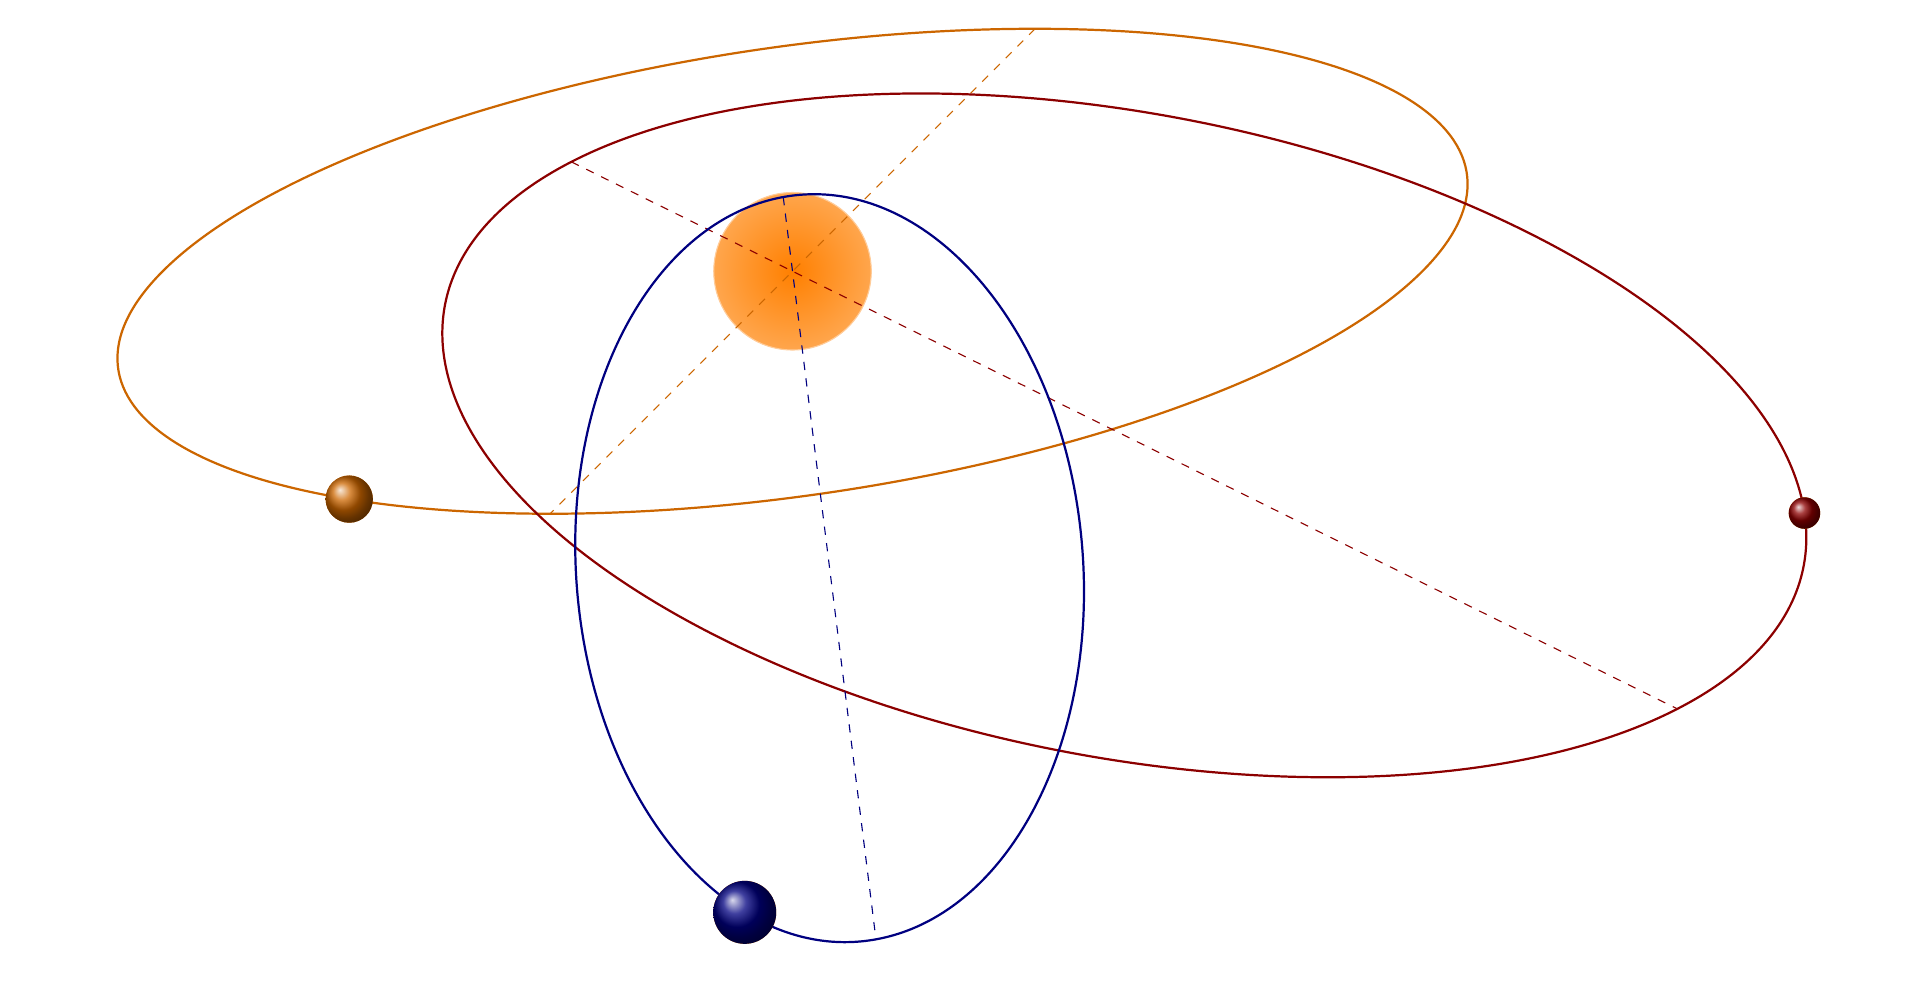
\begin{tikzpicture}[rotate around x=-90, rotate around z=-90]%, rotate around y=60]
    % \draw[->] (0,0,0) -- (1,0,0) node {$x$};
    % \draw[->] (0,0,0) -- (0,1,0) node {$y$};
    % \draw[->] (0,0,0) -- (0,0,1) node {$z$};


    \filldraw[sun] (0,0) circle (1cm);

    % \filldraw[sun] (0,0) circle (1.2cm);
    % \shade[ball color=orange] (0,0) circle(1cm);


    % \foreach \a/\b/\phi/\theta/\c in {
    %     5.0/4/0.0/0.0/mydarkorange,%
    %     8.0/3/20.0/0.0/mydarkred,%
    %     8.0/5/20.0/20.0/mydarkblue%
    % } {
    %     \pgfmathsetmacro{\e}{\a*(1 - \b^2 / \a^2)^.5}
    % \foreach \a/\eps/\phi/\theta/\c in {
    %     5.0/0/0.0/0.0/mydarkorange,%
    %     8.0/0.5/80.0/0.0/mydarkred,%
    %     4.0/0.6/30.0/45.0/mydarkblue%
    % } {
    %     \pgfmathsetmacro{\b}{\a*(1 - \eps^2)^.5}
    %     \pgfmathsetmacro{\e}{\a*\eps}


    %     \begin{scope}[
    %         rotate around z=\phi,
    %         rotate around y=\theta,
    %     ]
    %         \begin{scope}[
    %             canvas is xy plane at z=0,
    %             xshift=\e cm,
    %             \c,
    %         ]
    %             \draw[thick] (0,0) ellipse(\a cm and \b cm);

    %             \draw[innerline, \c] (-\a, 0) -- (\a, 0);
    %             \draw[innerline, \c] (0, -\b) -- (0, \b);

    %             \draw[foci] (-\e, 0) circle(0.04);
    %         \end{scope}
    %     \end{scope}
    % }
    
    \foreach \a/\eps/\incl/\longasc/\phiref/\c/\ppos/\psize in {
        8.0/0/0.0/0.0/0.0/mydarkorange/-20/0.3,%
        9.0/0.6/15.0/70.0/0.0/mydarkred/40/0.2,%
        5.0/0.8/45.0/30.0/0.0/mydarkblue/-30/0.4%
    } {
        \pgfmathsetmacro{\b}{\a*(1 - \eps^2)^.5}
        \pgfmathsetmacro{\e}{\a*\eps}


        \begin{scope}[
            rotate around z=\longasc,
        ]
            \begin{scope}[
                rotate around y=\incl,
                rotate around z=\phiref,
            ]
                \begin{scope}[
                    canvas is xy plane at z=0,
                    xshift=\e cm,
                    \c,
                ]
                    \draw[thick] (0,0) ellipse(\a cm and \b cm);

                    \draw[innerline, \c] (-\a, 0) -- (\a, 0);
                    % \draw[innerline, \c] (0, -\b) -- (0, \b);

                    % \draw[fill, \c!20!white, opacity=0.5] (0,0) ellipse(\a cm and \b cm);

                    % \draw[foci] (-\e, 0) circle(0.04);  % Verification


                    % \draw[body, \c] ({\a*cos(\ppos)}, {\b*cos(\ppos)}) circle(\psize cm);  % Circle gets rotated, too, not intended
                    % \coordinate (planet) at ({\a*cos(\ppos) cm}, {\b*sin(\ppos) cm});
                    
                    \pgfmathsetmacro{\x}{\a*cos(\ppos)}
                    \pgfmathsetmacro{\y}{\b*sin(\ppos)}
                    \coordinate (planet) at (\x cm, \y cm);
                \end{scope}
            \end{scope}
        \end{scope}

        % \draw[\c] (0, 0) -- (planet);  % For debugging
        % \draw[body, \c] (planet) circle(\psize cm);
        \shade[body, ball color=\c] (planet) circle(\psize cm);
    }

    % \filldraw[sun] (0,0) circle (1cm);  % In case ellipses are filled out

\end{tikzpicture}

\end{document}